% Diese Zeile bitte -nicht- aendern.
\documentclass[course=erap]{aspdoc}
\usepackage{amsmath}
\usepackage{pgfplots}

 %%%%%%%%%%%%%%%%%%%%%%%%%%%%%%%%%
 %% TODO: Ersetzen Sie in den folgenden Zeilen die entsprechenden -Texte-
 %% mit den richtigen Werten.
 \newcommand{\theGroup}{team 104} % Beispiel: 42
 \newcommand{\theNumber}{A325} % Beispiel: A123
 \author{Mikhail Lykov \and Viktor Bayo \and Georgy Chomakhashvili}
 \date{Wintersemester 2022/23} % Beispiel: Wintersemester 2019/20
 %%%%%%%%%%%%%%%%%%%%%%%%%%%%%%%%%

% Diese Zeile bitte -nicht- aendern.
\title{Gruppe \theGroup{} -- Abgabe zu Aufgabe \theNumber}

\begin{document}
\maketitle

\section{Einleitung}
 Die vorliegende Arbeit, die im Rahmen des Grundlagenpraktikums der Rechnerarchitektur durchgeführt wurde, widmet sich der Umsetzung eines Verfahrens zur Berechnung der Quadratwurzel von zwei mit beliebiger Genauigkeit. Dabei wurde ein Programm mit I/O-Operationen in C implementiert, mit welchen der Benutzer die Konstante in wählbarer Genauigkeit berechnen und wahlweise in dezimaler oder hexadezimaler Darstellung ausgeben lassen kann.
 
 Das Problem der Ermittlung mathematischer Konstanten gehört zu der Algorithmik, welche ein Teilgebiet der theoretischen Informatik ist, wobei die Letztere eine solide wissenschaftliche Basis bietet, um die zu dem Gebiet gehörigen Problemstellungen mathematisch zu lösen. Die Aufgabe, $\sqrt{2}$ mit beliebiger Genauigkeit effizient berechnen zu können, kann in engen Bereichen der Wissenschaft angewendet werden, wo die Genauigkeit der resultierenden Berechnungen sehr wichtig ist. Obwohl im alltäglichen Leben der Anspruch einer solchen Präzision nicht weit verbreitet ist, sind die Methoden, die für die entsprechenden Berechnungen verwendet werden, von grundlegender Bedeutung. Die Berechnung von $\sqrt{2}$ ist nicht trivial und erfordet daher eine solide theoretische Basis. Dies ermöglicht eine deutliche Gliederung der Aufgabe in zwei Teile: einen theoretischen Teil und eine praktische Umsetzung von Methoden.
 
 Im theoretischen Teil werden die benötigten Datenstrukturen und grundlegenden Methoden, auf denen weitere Berechnungen basieren, beschrieben und analysiert. Eine sorgfältige Wahl und Anpassung von Strukturen und Methoden trägt dazu bei, dass ein Programm schneller und zuverlässiger arbeitet. Dabei wird die Datenstruktur \texttt{struct bignum} realisiert, die alle notwendigen Eigenschaften besizt, um die Berechnung $\sqrt{2}$ mit beliebiger Genauigkeit erfolgreich zu machen. Danach werden die grundlegenden arithmetischen Operationen auf \texttt{struct bignum}, nämlich Addition, Subtraktion, Multiplikation und Division, realisiert. Um die Berechnungen zu beschleunigen, werden dabei Karazuba-Multiplikation und das Newton–Raphson-Verfahren für die Multiplikation und Division eingesetzt.
 
 Der praktische Teil besteht darin, das effektive Verfahren zur Berechnung von $\sqrt{2}$ ohne Genauigkeitsverlust zu implementieren. Hier werden die Binary Splitting-Methode, welche dazu beiträgt, die numerische Auswertung konvergenter Reihen zu beschleunigen, und das Newton-Raphson-Verfahren, ein Algorithmus zur Bestimmung von Nullstellen, untersucht. Das Newton-Raphson-Verfahren wird hier nicht nur als wirksame Methode für die Division zweier Zahlen verwendet, sondern auch zur Bestimmung des Wertes von $\sqrt{2}$ eingesetzt. Im Folgenden wird auch gezeigt, dass die in der Aufgabe vorgeschlagene Berechnung durch Binary Splitting nicht das effizienteste Verfahren ist. Darüber hinaus scheitert der Versuch, Berechnungen mit SIMD zu optimieren. Die Gründe werden in den jeweiligen Kapiteln beschrieben. Außerdem wurde es beschlossen, den Wert von $\sqrt{2}$ direkt im angegebenen Zahlensystem \texttt{base} zu berechnen, ohne eine Übertragung in das Binärsystem durchzuführen. Diese Entscheidung beruht auf den zusätzlichen Kosten, die bei der Konvertierung vom Binär- in das Dezimalsystem anfallen würden. Damit wird die Laufzeit des Algorithmus leicht beschleunigt.
 
\section{Lösungsansatz}
\subsection{Rahmenprogramm}
Der Code wird in mehrere Dateien, inklusive Header Dateien, aufgeteilt, um eine klare Struktur für die Interaktion zwischen Funktionen bereitzustellen. Das Rahmenprogramm nimmt bei einem Aufruf die in der Aufgabenstellung beschriebenen Optionen entgegen. Beim Analysieren der Eingabe-Randfälle wurde entschieden, dass das $-$ Zeichen nach $-h$ als der Beginn der nächsten Option gilt, sodass $-h$ keine negativen Werte annimmt, da negative Zahlen ungültige Eingabeparameter sind. Außerdem wird eine zusätzliche Option \texttt{-t <Zahl>} implementiert, um die automatischen Tests direkt beim Aufruf ausführen zu können,  gibt \texttt{--help} detaillierte Informationen und Beispiele. 

Die ursprünglich in der Aufgabenstellung spezifizierte Funktionssignatur wurde modifiziert und lautet nun \texttt{struct bignum sqrt2(size\_t s, numeral\_system\_t base)}. Dies geschah aufgrund der Entscheidung, Berechnungen  wählbar in Dezimal- oder Hexadezimalschreibweise  durchzuführen. Durch diese Gestaltung wurde die Notwendigkeit beseitigt, die Werte zweimal neu zu berechnen. Daher wird dieser Funktion die notwendige Anzahl an Nachkommstellen direkt im Körper der Funktion berechnet. Die Art und Weise der Umsetzung ist in dem Kapitel $"$Genauigkeit$"$ ausführlich beschrieben.

\subsection{Datenstruktur bignum}
Laut der Aufgabenstellung sollte eine Datenstruktur \texttt{struct bignum} definiert werden, um Ganzzahlen beliebiger Größe zu speichern. Zudem wurde ein Format für die Speicherung der Fixkommazahlen festgelegt. Die Gestaltung dieser Struktur wird in der Implementierung veranschaulicht und wird entsprechend mit sorgfältigen Kommentaren versehen. 

Die Grundidee der Datenstruktur \texttt{bignum} lässt sich konzeptionell wie folgt beschreiben: durch den ganzzahligen Teil namens \texttt{mantissa}, welcher durch Pointer auf ein Array von unsigned 8-bit Integers realisiert wird, und durch den Fixpunkt an der Position, die gleich \texttt{exponent} ist, welche durch einen signed 32-bit Integer repräsentiert wird. Laut Aufgabenstellung unterstützt die implementierte Datenstruktur die Dezimal- sowie Hexadezimal-Zahlensysteme. Das vorgeschlagene Format ermöglicht es, sowohl Ganzzahlen als auch Fixkommazahlen effizient zu speichern. Durch das Verwerfen führender und abschließender Nullen kann der Speicher effizient genutzt werden, was bei den anderen Gestaltungen nicht so einfach zu erreichen wäre. Das Format an sich erlaubt die Darstellung beliebiger Zahlen als $[0].mantissa \cdot basis^{exponent}$, was die Implementierung arithmetischer Operationen vereinfacht.

Die \texttt{bignum}-Struktur könnte auf verschiedene andere Arten definiert werden. Es ist jedoch sinnvoll, beide Zahlenmengen, sowohl Ganzzahlen als auch Fixkommazahlen, durch eine einzige Struktur darzustellen, da beide Typen für die Zwischenberechnungen benötigt werden. Das vorgeschlagene Format der \texttt{bignum}-Struktur ermöglicht es, alle erforderlichen arithmetischen Operationen in Integer-Arithmetik durchzuführen. Dabei reduziert sich die Abarbeitung der Punktposition nur auf die Korrektur von \texttt{exponent}.

Die Verwendung von Fließkommazahlen gemäß dem IEEE-754-Standard ist nicht geeignet, da der Wertebereich dieser Zahlen nicht das Kriterium der beliebigen Genauigkeit erfüllt. Wenn man beispielsweise die Darstellung von Fließkommazahlen mittels \texttt{double} betrachtet, so können betragsmäßig  Zahlen von ungefähr $10^{-308}$ bis $10^{308}$ dargestellt werden, was aber für die Aufgabe nicht genug sein kann. Somit wird gezeigt, dass das vorgeschlagene Format für die Datenstruktur \texttt{struct bignum} alle notwendigen Eigenschaften besizt, um die Berechnung von $\sqrt{2}$ erfolgreich zu machen.
\subsection{Arithmetik}
Um die Berechnung der Quadratwurzel aus zwei durchführen zu können, ist es notwendig, grundlegende arithmetische Operationen effizient für das Rechnen mit \texttt{bignum} zu realisieren. Die implementierten Funktionen können  mit Ganz- und Fixkommazahlen sowie mit negativen Zahlen gleichzeitig umgehen. Im Folgenden werden die entsprechende Lösungsansätze vorgestellt und analysiert, welche auf eine leistungsfähige Realisierung dieser Operationen abzielt.
\subsubsection{Addition und Subtraktion}
Für die effiziente Realisierung von Addition und Subtraktion(Subtraktion wird nicht explizit in der Aufgabestellung gefordert, aber ist für die Realisierung von Karazuba-Multiplikation und Newton–Raphson-Verfahren notwendig) kann man auf die klassischen Verfahren der Schulmathematik zurückgreifen. Zur Vereinfachung der Schreibweise wird die Notation: \texttt{a.exponent} = \texttt{a.exp}, \texttt{a.mantissa\_size} = \texttt{|a|} und \texttt{a.mantissa[i]} = \texttt{a[i]} verwendet. Um \texttt{a} + \texttt{b} = \texttt{result} zu realisieren, muss der entsprechende Stellenwert von \texttt{a} zum entsprechenden Stellenwert von \texttt{b} addiert werden, denn im allgemeinen Fall ist \texttt{a.exp} nicht gleich zu \texttt{b.exp}. 
Zur Ausrichtung der Ziffern werden die Variablen \texttt{a\_shift} und \texttt{b\_shift} verwendet, die beschreiben, um wie viel die Stellenwerte von \texttt{a} und \texttt{b} relativ zum Antwortergebnis verschoben werden müssen. Dabei gilt: $|result| = max(|a| + a\_shift), |b| + b\_shift)$ und $result.exp = max(a.exp, b.exp)$. Damit sieht die Addition von zwei \texttt{bignums} schematisch wie folgt aus, wobei $a = 13.4$ und $b = 0.25$:

\begin{equation}
\begin{tabular}{c@{\;}c@{\;}c@{\;}c@{\;}c}
  & 0 & 0 . & 0 & 0 \\
+ & 1 & 3 . & 4  \\
\hline
  & 1 & 3 . & 4 & 0 \\
+ &   & 0 . & 2 & 5 \\
\hline
  & 1 & 3 . & 6 & 5 \\
\end{tabular}
\end{equation}
Um zwei Zahlen \texttt{a} und \texttt{b} analog zu subtrahieren, müssen auch die entsprechenden Stellenwerte von \texttt{b} von den entsprechenden Stellewerten von \texttt{a} subtrahiert werden. Dabei benuzt man wieder \texttt{a\_shift}, \texttt{b\_shift} auf die gleiche Weise. Allerdings ist hier ein Sonderfall möglich, wenn $a < b$. Um diesen Sonderfall zu beheben, fügt man $1$ vor den höheren Stellenwert im Ergebnis ein. Wenn diese 1 nach der Subtraktion verschwunden ist, bedeutet dies, dass $a < b$ war. Als Antwort kriegt man dann die Differenz dieser Zahlen, aber im Double Compliment. Anderfalls war $a \geq b$ und die Differenz erhält man in direkter Form. Zum Beispiel:
\begin{equation}
\begin{tabular}{c@{\;}c@{\;}c@{\;}c@{\;}c@{\;}c}
  & [1] & 0 & 0 . & 0 & 0 \\
+ & & 1 & 3 . & 4  \\
\hline
  & 1 & 1 & 3 . & 4 & 0 \\
- & & & 0 . & 2 & 5 \\
\hline
  & [1] & 1 & 3 . & 1 & 5 \\ 
\end{tabular}
\\ \quad \quad \quad \quad
\begin{tabular}{c@{\;}c@{\;}c@{\;}c@{\;}c@{\;}c}
  & [1] & 0 & 0 . & 0 & 0 \\
+ & & & 0 . & 2 & 5 \\
\hline
  & 1 & 0 & 0 . & 2 & 5 \\
- & & 1 & 3 . & 4  \\
\hline
  & [ ] & 8 & 6 . & 8 & 5 \\ 
\end{tabular}
\\ 
\begin{tabular}{c@{\;}c}
  &  \\
  &  \\
  &  \\
  &  \\
  & $\implies -13.15$ \\
\end{tabular}
\end{equation}

\subsubsection{Multiplikation}
Da man im Rahmen dieser Aufgabe sehr große Zahlen effizient multiplizieren muss, erfordert daher die Berechnung zusätzlichen Aufwand. Betrachten wir nun die naive Multiplikation zweier Zahlen mittels Schulmethode. Um zwei Zahlen \texttt{a} und \texttt{b} auszumultiplizieren, multipliziere \texttt{a} mit jeder Ziffer von \texttt{b} und addiere anschließend die Teilprodukte. In diesem Fall führt es insgesamt zu einer Laufzeitkomplexität von $\Theta(n^2)$. 

Beim Multiplizieren wird Integer-Multiplikation von Mantissen beider Zahlen durchgeführt: Die aufaddierten Exponenten werden am Ende dem Ergebnis zugewiesen. Es ist offensichtlich, dass $|result| = |a| + |b|$. Dabei kann der Koeffizent result[i] im Allgemeinen, wie links \ref{eq:mult} dargestellt, berechnet werden. Es ist aber wichtig, dass Koeffizent $i$ und $i - j$ muss in die Grenzen von beiden Zahlen sein. Dabei werden \texttt{l} und \texttt{r}  so gewählt, dass $0 \leq j \leq |a| - 1$ und $0 \leq (i - j) \leq |b| - 1 $. Daher muss die Gleichung modifiziert werden:
\begin{equation}
result[i] = \sum_{j=0}^i {a[j] \cdot b[i - j]} \\ \quad \implies \quad
result[i] = \sum_{j=l}^r {a[j] \cdot b[i - j]}
\label{eq:mult}
\end{equation}
Eine vektorisierte Version der naiven Multiplikation wurde ebenfalls implementiert. Es wird dabei versucht, 8 Werte gleichzeitig zu multiplizieren, wobei sie zu einem Vektor hinzugefügt werden, um die Laufzeit der Berechnung zu beschleunigen. Jedoch hat diese Vektorisierung das Programm nur verlangsamt. Daher wird die Funktionsweise der vektorisierten Multiplikation als technischer Aspekt betrachtet und wird nicht in dieser Arbeit beschrieben.

\subsubsection{Karazuba-Multiplikation} 
Allerdings ist die naive Multiplikation für die gewünschte Laufzeit unseres Programms zu langsam. Diese lässt sich mittels Divide-and-Conquer Methode reduzieren, beispielsweise mittels des Karazuba-Algorithmus. Die Idee ist, eine Multiplikation mit n-stelligen Zahlen in drei Multiplikationen mit Zahlen der Länge n/2 + $\mathcal{O}(n)$ zusätzlichem Aufwand um die Operationen auf Zwischenergebnisse aufzuteilen. Dabei reduziert sich die Laufzeit der Multiplikation von $\mathcal{O}(n^{2})$ auf $\mathcal{O}(n^{1.59})$. Der Algorithmus wird rekursiv aufgerufen und auf jeder Rekursionsebene werden die Zahlen bezüglich ihrer Länge halbiert. Die Funktion wird solange rekursiv aufgerufen bis eine der Zahlen (oder beide) klein genug ist um direkt naiv multipliziert zu werden. Darüber hinaus werden die Besonderheiten der Anwendung des Karazuba-Algorithmus auf die \texttt{bignum}-Datenstruktur dargestellt. Die halbe Länge der Zahlen wird wie folgt berechnet: $half\_size = \left\lceil |a|/2 \right \rceil$.

Ausgehend davon, dass jede \texttt{bignum} als $[0].mantissa \cdot basis ^{exponent}$ dargestellt werden kann, können \texttt{a} und \texttt{b} so \ref{eq:ab} dargestellt werden, wobei $ah / bh $ die obere Hälfte der Zahl, $al / bl$ die niedere Hälfte der Zahl und  $base$ das gegebene Zahlsystem ist:
\begin{equation} 
a = ah + al \cdot base ^ {-half\_size} \quad \text{und} \quad
b = bh + bl \cdot base ^ {-half\_size}
\label{eq:ab}
\end{equation}
Auf diese Weise erhält man eine Formel, mit welcher der Karazuba-Algorithmus für beliebig große Zahlen implementiert werden kann. Bei der Entwicklung der Implementierung fiel es auf, dass bei kleinen Längen von \texttt{a} und \texttt{b} die naive Multiplikation schneller funktionierte als die Multiplikation nach der Karazuba-Methode. Anstatt Zahlen bis zur Länge 1 zu halbieren, wird dementsprechend, wenn die Länge der kleineren von beiden Zahlen 32 ist, die naive Multiplikation verwendet.
Dann wird $a \cdot b$  zu: 
\begin{equation} ah \cdot bh + ((ah + al)(bh + bl) - ah \cdot bh - al\cdot bl) \cdot base^{-half\_size} + al \cdot bl\cdot base^{-2 \cdot half\_size} \end{equation}\subsubsection{Division}
In diesem Abschnitt wird die Vorgehensweise zur Realisierung der Division mit einer \texttt{n}-stelligen Genauigkeit erläutert. Hierbei entspricht \texttt{n} der Anzahl von den \texttt{mantissa}-Stellen im Ergebnis der Division im gegebenen Zahlenformat. Dabei betrachet man die Division der Zahl \texttt{a} durch die Zahl \texttt{b} als die Multiplikation von \texttt{a} mit einem Kehrwert(engl. reciprocal) $1/b$. Dank dem \texttt{bignum}-Format kann das Ergebnis der Division als die Mantissendivision, multipliziert mit $basis^{a.exp - b.exp}$ dargestellt werden. Die Berechnung des Kehrwerts, die mithilfe des Newton-Raphson-Verfahrens approximiert wurde, wird im nachfolgenden Kapitel dargestellt.


\subsubsection{Newton-Raphson-Verfahren}
Das Newton-Raphson-Verfahren ~\cite{Newton-Raphson-Verfahren} ist ein Algorithmus  zum Finden von Nullstellen von stetigen Funktionen. Da im Allgemeinen die Nullstellen einer Funktion nicht exakt berechnet werden können, liefert dieses Verfahren keine exakte Lösung sondern die Annäherung an die Nullstelle. Das Newton-Raphson-Verfahren verwendet Iterationen und erzeugt eine Folge von Zahlen, die gegen die Nullstellen konvergiert. Es erfordert außerdem eine anfängliche Schätzung $x_{0}$ als Startwert. Dabei erzeugt jede Iteration des Algorithmus eine sukzessive genauere Approximation. Bei erfolgreicher anfänglicher Schätzung verdoppelt sich (fast) die Anzahl der korrekten Stellen bei jedem Schritt der Iteration. Der Vorgang wird solange wiederholt, bis ein ausreichend genauer Wert erreicht ist, nämlich bis die Anzahl von Nachkommastellen des Kehrwertes größer als der übergebene Parameter \texttt{n} ist. Die Formel zur Berechnung der nächsten Approximation sieht folgendermaßen aus, wobei $i\in\mathbf{N} $ und $x_{i + 1}$ immer eine bessere Approximation als $x_{i}$ ist: 
\begin{equation}
x_{i + 1} =  x_{i} - \frac{f(x_{i})}{f'(x_{i})} 
\label{eq:nächste Näherung}
\end{equation}
Um eine präzise Annäherung des Kehrwerts zu erhalten, musste eine geeignete stetige Funktion ausgewählt werden, die beim Einsatz von $1/b$ eine Null liefert. Somit sieht unsere Funktion folgendermaßen aus: $f(x) = 1/x - b$. Wird die obige Formel auf die vorgeschlagene Funktion angewendet, erhält man den folgenden Ausdruck: 
\begin{equation} x_{i + 1} = x_{i} - \frac{1/x-b}{-1/x^{2}} = x_{i} * (2 - b *  x_{i}) = x_{i} + (1 - b * x_{i}) * x_{i} 
\label{eq:Konvergenzformel}
\end{equation}
Aufgrund der Besonderheit unserer Implementierung: wenn $b \in [0.1, 1]$, dann $(1/b) \in [1, basis]$. Folglich darf man die anfängliche Schätzung $x_{0} = 1$ nehmen. Die Genauigkeit der gesamten Approximation kann mittels Ausdruck $(1 - b * x_{i}) * x_{i}$ verfolgt werden und wird \texttt{residual} genannt. Der Algortihmus stoppt, wenn $|residual.exp| > n$ ist. 

Da \texttt{bignum} keine Verluste an Genauigkeit aufweist, wächst die Länge von $x_{i}$ bei der Berechnung der Annäherungen sehr schnell, was zu einer deutlichen Verlangsamung des Algorithmus führt. Um diesem Problem entgegenzuwirken wurden die unteren Stellen von $x_{i}$ verworfen. Es wurde beschloßen, dass Stellenwerte mit einem Wert kleiner als $2 \cdot |\texttt{residual.exponent}| + 4$ verworfen werden sollten. Diese Konstante wurde so gewählt, da das Newton-Verfahren die Anzahl der korrekt berechneten Stellen pro Iterationsschritt ungefähr verdoppelt. Aufgrund dieser Überlegungen kann man schlussfolgern, dass dieser Trick den Algorithmus nicht bricht, aber ihn beschleunigt.

Die Laufzeitskomplexitat des Newton-Raphson-Verfahrens kann wie folgt analysiert werden: Sei $t(n)$ die Division mit einer Genauigkeit von \texttt{n} Stellen. $t(n) = t(n/2) + O(M(n))$, wobei \texttt{n} die Länge der Zahlen im aktuellen Schritt  und $M(n) = O(n^{1.59})$  die Multiplikationszeit ist. Nach  dem Master-Theorem gilt: $t(n) = O(n^{1.59})$.

\subsection{Berechnung der Konstante}
Laut der Projektaufgabe ist die Approximation der mathematischen Konstante $\sqrt{2}$ mit beliebiger Genauigkeit \texttt{effizient} zu berechnen. Demgemäß werden zwei Vorgehen zur Berechnung vorgeschlagen: Eine Auswertung mittels Binary Splitting und eine Approximation mittels Newton-Raphson-Verfahren. In diesem Abschnitt wird die Verwirklichung beider Vorgehen betrachtet. Danach werden die besprochenen Ansätze anhand ihrer Genauigkeit und Perfomanz in den entsprechenden Kapiteln analysiert.

\subsubsection{Berechnung mittels Binary Splitting} 
In der Mathematik ist Binary Splitting eine Technik zur Beschleunigung der numerischen Auswertung vieler Arten von Folgen mit rationalen Termen. Insbesondere ist Binary Splitting auf konvergente Reihen der folgenden Form anwendbar ~\cite{BinarySplitting} :
\begin{equation}
S = \sum_{n=1}^{\infty} \frac{a(n)}{b(n)} \cdot \frac{p(1)...p(n)}{q(1)...q(n)}
\label{eq:reihe}
\end{equation}
Aus der Aufgabenstellung ist bekannt, dass die mathematische Konstante $\sqrt{2}$ in folgender Form darstellbar ist:
\begin{equation} 
\sqrt{2} = 1 + \sum_{i=1}^{\infty} \prod_{k=1}^i \frac{2k - 1}{4k} 
\label{eq:reihe1}
\end{equation}
Dann kann die Formel \ref{eq:reihe1} durch Formel \ref{eq:reihe}  unter Verwendung der folgenden Polynome dargestellt werden:
$a(n) = 1$, $b(n) = 1$, $p(n) = 2n - 1$ und $q(n) = 4n$. Um $\sqrt{2}$ mittels Binary Splitting zu berechnen, müssen außerdem die folgenden Formeln ausgedrückt werden:
\begin{equation} 
S_{n_{1}, n_{2}} = \sum_{n = n_{1}}^ {n_{2} - 1} {\prod_{k = n_{1}}^{n} \frac{2k - 1}{4k}} \quad \quad \quad 
P_{n_{1}, n_{2}} = \prod_{k = n_{1}}^{n_{2} - 1} {2k - 1}
\end{equation}
\begin{equation} 
Q_{n_{1}, n_{2}} = \prod_{k = n_{1}}^{n_{2} - 1} {4k} \quad \quad \quad  \quad \quad \quad 
T_{n_{1}, n_{2}} = Q_{n_{1}, n_{2}} \cdot S_{n_{1}, n_{2}}
\end{equation}
Da $\sqrt{2}$ durch die Reihe\label{reihe} dargestellt werden kann, ist es es möglich, $T_{n_{1}, n_{2}}$ rekursiv auszudrücken. Daher konnte zuerst $T_{n_{1}, n_{2}}$ in Bezug auf kleinere $T$, $Q$ und $P$ berechnet werden:
\begin{equation} 
T_{n_{1}, n_{2}} = 
\begin{cases}
 p(n_{1}) = 2 n_{1} - 1 & \text{if $n_{1} = n_{2} - 1$,}\\
T_{n_{1}, m}  \cdot Q_{m, n_{2}} + P_{n_{1}, m} \cdot T_{m, n_{2}} & \text{otherwise, wobei $m = \left \lfloor \frac{n_{1} + n_{2}}{2} \right \rfloor$}
\end{cases}
\label{eq:T}
\end{equation}
Dank dieser Darstellung kann man $S_{n_{1}, n_{2}}$ aus Formel \ref{eq:T} durch $T_{n_{1}, n_{2}}$ ausdrücken:
\begin{equation} 
S_{n_{1}, n_{2}} = \frac{T_{n1, n2}}{Q_{n1, n2}}
\end{equation} 
Als Ergebnis muss dann $S_{1, n}$ für ein gegebenes $n$ berechnet werden, da $S_{1, n} \approx \sqrt{2} - 1$ ist. Dazu müssen  $T_{1, n}$ und $Q_{1, n}$ berechnet werden. Zu beachten ist, dass $P_{n_{1}, n_{2}}$ und $Q_{n_{1}, n_{2}}$ benötigt werden, um die Funktion T zu berechnen. Daher werden parallel zur Berechnung von $T$ $P_  {n_{1}, n_{2}}$ und $Q_{n_{1}, n_{2}}$ auch rekursiv berechnet, weil $P{n_{1}, n_{2}}$ = $P_{n_{ 1}, m} \cdot P_{m, n_{2}}$ und $Q_{n_{1}, n_{2}}$ = $Q_{n_{1}, m} \cdot Q_{ m, n_ {2}}$.

Die Laufzeitkomplexitat kann wie folgt analysiert werden: Sei $t(n)$ die Laufzeit von $T_{1, n}$ , dann ist $t(n) = 2 \cdot t(n/2) + \mathcal{O}(M(n\log{n}))$, wobei $n\log{n}$  die resultierende Länge der Zahlen $T$, $Q$ und $P$ im aktuellen Schritt ist. $M(n\log{n}) = (n\log{n}) ^ {1.59}$ - Laufzeit der Multiplikation. Dann gilt nach dem Master-Theorem: $t(n) = \mathcal{O}((n\log{n}) ^ {1,59})$ .

\subsubsection{Berechnung mittels Newton-Raphson-Verfahren} 
Es ist interessant festzustellen, dass das von der Aufgabenstellung vorgeschlagene Newton-Raphson-Verfahren so mächtig ist, dass es  auch direkt zur Approximierung von $\sqrt{2}$ verwendet werden kann. Genau diese Eigenschaft der Methode wird verwendet, um die Berechnung von $\sqrt{2}$ in der Optimierung zu beschleunigen. Da die Funktionsweise des Newton-Raphson-Verfahrens bereits zuvor schon erklärt wurde, werden im Folgenden nur die Feinheiten zur Approximation von $\sqrt{2}$ betrachtet. Wählt man nun eine stetige Funktion, welche beim Einsetzen von $\sqrt{2}$ eine Null liefert: $f(x) = x^{2} - 2$. Die anfängliche Schätzung ist  $x_{0} = 1$, da $\sqrt{2} \ge 1$. Wird die Formel \ref{eq:nächste Näherung} auf die vorgeschlagene Funktion angewendet, erhält man den folgenden Ausdruck: \begin{equation} x_{i+1} = x_{i} - \frac{x^{2} - 2}{2x} = x_{i} + \frac{1}{2} \left(\frac{2}{x_{i}} - x_{i}\right)  \end{equation}
Ähnlich wie bei dem obigen Verfahren hat hier \texttt{residual} = $\frac{1}{2} \left(\frac{2}{x_{i}} - x_{i}\right)$ die gleiche Funktion wie bei der Berechnung vom Kehrwert. Der Hauptunterschied bei dieser Annäherung ist die Notwendigkeit, $2/x_{i}$ zu dividieren. Dazu müssen wir die erforderliche Anzahl von Zeichen für die Genauigkeit bestimmen, mit der $2/x_{i}$ gezählt wird. Wissend, dass das Newton-Raphson-Verfahren die Anzahl der richtigen Zahlen pro Iterationsschritt (fast)verdoppelt, muss $2/x_{i}$ mit einer Genauigkeit von mindestens $2 \cdot|residual.exponent| + 4$ berechnet werden.

Die Laufzeitkomplexitat kann wie folgt analysiert werden: $ t(n) = t(n/2) + \mathcal{O}(D(n))$, wobei \texttt{n} die Länge der Zahl im aktuellen Schritt und $D(n) = \mathcal{O}(n^{1.59})$. Nach dem Master-Theorem gilt: $t(n) = \mathcal{O}(n^{1.59})$

% TODO: Je nach Aufgabenstellung einen der Begriffe wählen
\section{Genauigkeit}
 Die Genauigkeit der Berechnung von $\sqrt{2}$ hängt von der Anzahl der gewünschten binären Nachkommastellen ab. Das in der Hauptimplementierung benutzte Binary Splitting erhält als Eingabeparameter außerdem die Variablen $from$ und $to$. $from$ wird dabei immer mit 1 initialisiert und wie man $to$ wählen soll, ist im Weiterem beschrieben. 

 Aus dem obigen Kapitel ist schon bekannt, dass $\sqrt{2} = 1 + S_{1, to}$, wobei $to$ richtig gewählt werden muss, um eine ausreichend präzise Genauigkeit zu gewährleisten. Betrachten wir dazu die Formel \ref{eq:reihe1}. Lasst uns ein Element dieser Summe schätzen:
\begin{equation} 
\prod_{k = 1}^{i} {\frac{2k-1}{4k}} = \frac{1}{4}\prod_{k = 2}^{i} \frac{2k-1}{4k} \leq \frac{1}{4} \prod_{k = 2}^{i} \frac{2k}{4k} = \frac{1}{4}\prod_{k = 2}^{i} \frac{1}{2} \leq \Bigl(\frac{1}{2}\Bigr)^{i+1}
\end{equation}
Dann lasst sich die Berechnungsfehler folglich schätzen: 
\begin{multline}
\sqrt{2} - (1 + S_{1, to}) 
 = 1+\sum_{i=1}^{\infty}\prod_{k=1}^{i}\frac{2k-1}{4k}-(1+S_{1,to})=\\
 = \sum_{i=to}^{\infty}\prod_{k=1}^{i}\frac{2k-1}{4k} 
 \le \sum_{i=to}^{\infty} \Bigl(\frac{1}{2}\Bigr)^{i+1} = \Bigl(\frac{1}{2}\Bigr)^{to} 
\end{multline}
Mit anderen Worten, hat das oben beschriebene $S_{1, to}$  eine Genauigkeit bis $to-1$ Binärstellen. Da die gewünschte Anzahl von Nachkommastellen $s$ vom Nutzer in Bezug auf Dezimal- oder Hexadezimalsystem übergeben wird, müsste dann $to$ in Abhängigkeit vom übergegebenen Zahlensystem wie unten gezeigt berechnet werden. Es wird extra eins dazu aufaddiert, um sicherzustellen, dass die ersten $to$ Stellen  ohne Fehler berechnet werden.
\begin{itemize}
    \item Dezimalsystem: 1 Dezimalstelle erfordert  10/3 Binärstellen. 10 Bit reichen aus, um 3 Dezimalstellen zu speichern ( $2^{10} > 10^{3}$). $to = 
    \left\lceil (10\cdot s) / 3 \right \rceil + 1$. 
    \item Hexadezimalsystem: 1 Hexadezimalstelle erfordert 4 Binärstellen. 4 Bit werden benotigt, um 1 Hexadezimalstelle zu speichern. $to = 4\cdot s + 1$.
\end{itemize}
Zur Überprüfung der Fähigkeit der implementierten Funktionen genaue Berechnungen durchführen zu können und damit korrekte Ergebnisse zu liefern, werden automatisierte Tests realisiert. Die Beschreibung dieser Tests wird in der Dokumentation in Implementierung beschrieben.

\section{Performanzanalyse}
 Um die Performanz der Implementierungen für die Berechnung der Konstante $\sqrt{2}$ in der vorliegenden Arbeit zu testen, wurden die automatisierten Tests mit Benchmarking dementsprechend erweitert. Die automatisierten Tests dienen dazu, die Methoden zur Messung und Selektion von schwankenden Werte nachvollziehbarer zu machen. Getestet wurde auf einem System mit einem Quad-Core Intel Core i5 Prozessor, 1,1 GHz, 16 GB Arbeitsspeicher, MacOS Ventura 13.1 (22C65), 64 Bit, 22.2.0 Darwin Kernel Version 22.2.0. Kompiliert wurde mit Apple clang version 14.0.0 mit der Option -O3. Die Zeit wurde mithilfe der \texttt{clock\_gettime} und \texttt{CLOCK\_MONOTONIC} gemessen, wie von den Materialien auf der Praktikums-Website vorgeschlagen.  Irrelevante Operationen wie I/O oder Codeteile, die nichts mit der Berechnung $\sqrt{2}$ zu tun haben werden nicht mitgemessen. Für eine genaue Zeitmessung wurde durch die mehrmalige Ausführung gewährleistet, dass zwischen Messpunkten mindestens 1 Sekunde liegt. Eine Iterationsanzahl kleiner als 3 wird auch für sehr große Testwerte nicht zugelassen. Um die durchschnittliche Dauer eines Funktionsaufrufes zu erhalten , wird die Gesamtdauer anschließend durch die Anzahl der Iterationen geteilt. Um aussagekräftige Ergebnisse zu erhalten, wurde außerdem für jede Implementierung drei Messungen durchgeführt und dann der Median aller Durchschnitte als tatsächlich ermitteltes Ergebnis genommen. Da es keine stark abweichenden Ergebnisse gab, wurde entschieden, die Ergebnisse automatischer Messungen in dieser Arbeit mittels dieser Grafik \ref{chart:zeitmessungen} darstellen zu lassen. Die x-Achse ist dabei die Anzahl an dezimalen Nachkommatellen $\times 10 ^ {3}$. Zur bessere Darstellung werden hier die Werte von 100 bis 55000 angezeigt. Die y-Achse zeigt dabei die Laufzeit in Sekunden. In dieser Arbeit werden die Messungsergebnisse nur für die Dezimalwerte dargestellt, um nicht zwei identische Graphen zu zeigen. Jedoch wird es vermuten, dass Benchmarking für die großere Hex-Werte wird langsamer wegen Anzahl der Nachkommastellen.
 Für die Überprüfung der Performanz der Berechnung von $\sqrt{2}$ wurde auf verschiedene Vergleichsimplementierungen zurückgegriffen. Die Hauptimplementierung(Version 0) mit Binary Spiltting und der naiven Multiplikation diente dabei als Einstieg. Beim nächsten Schritt wurde vesucht, den langsamsten Teil des Codes zu finden und entsprechend zu optimieren. Mit Hilfe von Profiling wurde festgestellt, dass die naive Multiplikation den größten Teil der Arbeit des gesamten Algorithmus ausmacht. Aus diesem Grund wurde entschieden, die Multiplikation mittels SIMD-Instruktionen zu optimieren. Leider hat diese Vektorisierung das Programm nur verlangsamt. Die Überprüfung des generierten Assemblercodes zeigte, dass der Compiler mit der Option -O3 die Multiplikation selbst vektorisierte und zwar effizienter als wir. Es wird angenommen, dass die Beschleunigung durch Vektorisierung im Code durch zusätzliche Kosten für Konstruktion von Vektoren aus \texttt{bignum} nivelliert wurde. Aus diesem Grund wurde entschieden, dass die Optimierung von Berechnungen mit SIMD nicht den gewünschten Speedup bringt und daher weitere Optimierungen auf diese Weise nicht durchgeführt werden. Vektorisierte Multiplikation wird trotzdem für Überprüfungszwecke verwendet und als Bestätigung auch gemessen(Version 1). Um die Zeitmessungen zwischen der Hauptimplementierung und der Optimierung mittels Newton-Raphson-Verfahren(Version 2) zu analysieren, wird vorgeschlagen, sich auf Grafik \ref{chart:zeitmessungen} zu beziehen.
\begin{figure}
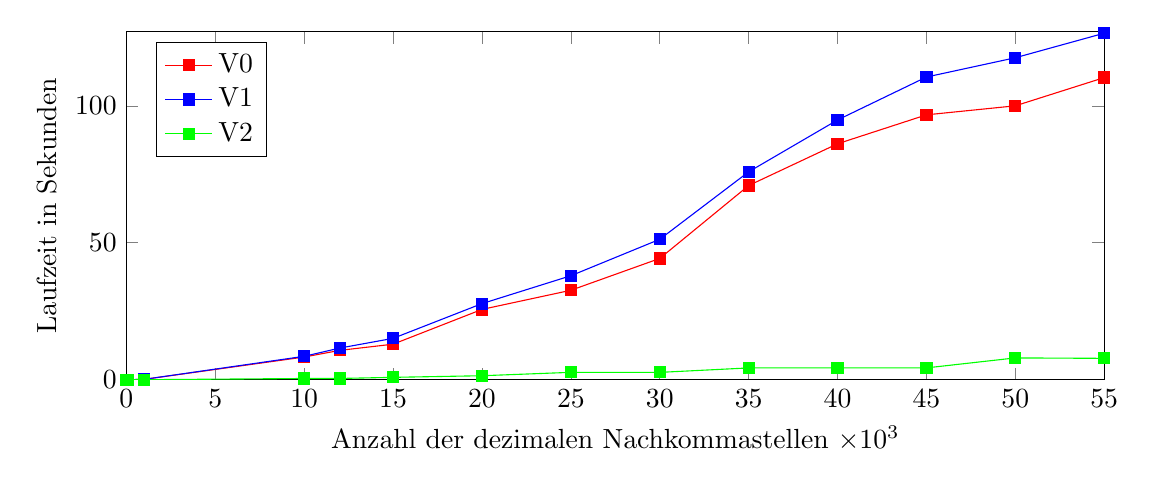
\begin{tikzpicture}
\begin{axis}[
    xlabel={Anzahl der dezimalen Nachkommastellen $\times 10^{3}$},
    ylabel={Laufzeit in Sekunden},
    xmin=0, xmax=55,
    ymin=0, ymax=127,
    width=14cm, height=6cm,
    legend pos=north west,
]
\addplot[color=red, mark=square*,] %VERSION_0 DEC
    coordinates { 
    (0, 0) 
    (0.1, 0.001776)
    (1, 0.136115)
    (10, 8.287759) 
    (12, 10.717704)
    (15, 12.974279)
    (20, 25.666717)
    (25, 32.655881)
    (30, 44.274327)
    (35, 70.882403)
    (40, 86.130601)
    (45, 96.692306)
    (50, 99.988629)
    (55, 110.291935)
    };
    
\addplot[color=blue, mark=square*,] %VERSION_1 DEC
    coordinates { 
    (0, 0) 
    (0.1, 0.002013)
    (1, 0.147009)
    (10, 8.551532) 
    (12, 11.556203)
    (15, 15.103992)
    (20, 27.784771)
    (25, 37.960783)
    (30, 51.265395)
    (35, 75.892572)
    (40, 94.822493)
    (45, 110.496426)
    (50, 117.536233)
    (55, 126.491935)
    };

\addplot[color=green, mark=square*,] %VERSION_2 DEC
    coordinates { 
    (0, 0) 
    (0.1, 0.000358)
    (1, 0.009923)
    (10, 0.454588) 
    (12, 0.466238)
    (15, 0.874035)
    (20, 1.461005)
    (25, 2.697679)
    (30, 2.683120)
    (35, 4.307987)
    (40, 4.331893)
    (45, 4.321101)
    (50, 7.962622)
    (55, 7.807733)
    };
\legend{
V0, 
V1,
V2,
}
\end{axis}
\end{tikzpicture}
\caption{Zeitmessungen der Berechnung $\sqrt{2}$}
\label{chart:zeitmessungen}
\end{figure}

 Anhand der Messungen ist ersichtlich, dass die Berechnung von $\sqrt{2}$ mittels Newton-Raphson-Verfahren um ein Vielfaches schneller als die Berechnung mittels Binary Splitting ist, was durch theoretische Berechnungen der Laufzeitkomplexität beider Verfahren bestätigt wird: Newton-Raphson-Verfahren  - $\mathcal{O}(n^{1.59})$, Binary Splitting - $\mathcal{O}((n\log{ n})^{1.59})$. Das Problem von Binary Splitting besteht darin, dass um die \texttt{n} Stellen berechnen zu können, die Polynome mit $n\log{n}$ Stellen berechnet werden müssen. Aber im Fall des Newton-Raphson-Verfahrens bleiben alle Zwischenwerte in der Größenordnung von \texttt{n} Stellen. Bereits bei kleinen Werten wird dieser Unterschied deutlich signifikanter.
 
Die Ausbuchtung im Graph kann auch auf die Struktur des Binary Splitting zurückgeführt werden. Da bei jedem Schritt das aktuelle Segment halbiert wird, ist die Rekursionstiefe gleich $\lceil\log^{2}{n}\rceil$. Dementsprechend hängt die Laufzeit des Algorithmus von diesem Wert ab. Man sieht leicht, dass $\lceil\log^{2}{n}\rceil$ für alle $n \in (2^{k} + 1,  2^{k + 1})$ gleich ist. Das führt dazu, dass innerhalb dieses Segments ein flacherer Graph und Sprünge zwischen diesen Segmenten zu beobachten sind. 

Da das Benchmarking auf große Werte ziemlich lange dauert, kann man nur grob (Anhand der Dezimal-Ergebnisse)abschätzen, wie lange das Programm braucht, um die ersten $10^{6}$ Nachkommastellen zu berechnen. Dabei werden separat Messungen für 100000 dezimale Nachkommastellen durchgeführt. Die Hauptimplementierung brauchte 366.741098 Sekunden und Version 2 brauchte 30.627304 Sekunden. Setzt man die bereits erhaltenen Messungsergebnisse in die vorberechnete Laufzeitskomplexität ein, so erhält man den Koeffizienten für die Hauptimplementierung: $8.24 \cdot 10 ^ {-7} \implies$ ungefähr 17142 Sekunden und Version 1: $3.48 \cdot 10 ^{-7} \implies$ ungefahr 1200 Sekunden. Solche grobe Schätzung macht deutlich, dass man auf das Ergebnis von Messungen für $10^{6}$ Nachkommastellen ungefähr 14 Stunden warten muss.

\section{Zusammenfassung und Ausblick}
In dieser Arbeit wurde eine Datenstruktur präsentiert, die zur effizienten Speicherung von Zahlen beliebiger Größe und zur Verwaltung von Fixkomma- Berechnungsergebnissen entwickelt wurde. Die Eigenschaften dieser Datenstruktur wurden analysiert und auf die Berechnung von $\sqrt{2}$ angewendet. Um mit diesem Format genaue und schnelle Berechnungen durchführen zu können, wurden die grundlegenden arithmetischen Operationen ausführlich beschrieben und in die Praxis umgesetzt. Außerdem wurde auch eine schnelle Multiplikation großer Zahlen nach der Karazuba-Methode implementiert. Der Versuch, die Multiplikation durch Vektorisierung zu beschleunigen, schlug fehl. Das Newton-Raphson-Verfahren, welches als effizientes Verfahren für die Division vorgeschlagen wurde, wird auch zur direkten Berechnung der Wurzel verwendet. Dessen Verwendung in unserer Arbeit dient jedoch nur als Vergleichsimplementierung. Letztlich wurde Binary Splitting für die Berechnung angewendet. Die Relevanz seiner Anwendung bei Berechnungen, die eine hohe Genauigkeit erfordern, wurde mathematisch bewiesen. Insgesamt wurden die drei beschriebenen Versionen in Bezug auf ihre Perfomanz verglichen. Insgesamt stellt sich heraus, dass das Newton-Raphson-Verfahren  eine effiziente und präzise Methode ist $\sqrt{2}$ zu berechnen. Damit ist in der Aufgabe vorgeschlagene Berechnung mittels Binary-Splitting nicht die effektivste Methode. 

% TODO: Fuegen Sie Ihre Quellen der Datei Ausarbeitung.bib hinzu
% Referenzieren Sie diese dann mit \cite{}.
% Beispiel: CR2 ist ein Register der x86-Architektur ~\cite{intel2017man}.
\bibliographystyle{plain}
\bibliography{Ausarbeitung}{}

\end{document}
